\documentclass[twoside, a4paper]{article}
\usepackage{amsmath}
\usepackage{float}
\usepackage{graphicx}
\newfloat{program}{thp}{lop}
\floatname{program}{Listing}
\author{Lukas Hofmaier}
\title{Type class laws}

\begin{document}
\maketitle
\tableofcontents

\section{Introduction}
\label{sec:intro}

Formal verification is a tool use for software application with the aim of providing a high reliability. The first formally verfified microkernel, seL4 was verified using Haskell. Haskell was used because programmers can reason about the source code \cite{Klein09}. Correctness is specified in form of equations. The source code must satisfy this equations. Programmers can use equational reasoning to verify the correctness of these equations.
Purely functional programming languages are easier to reason about as imperative or object-oriented languages.

\section{Type classes}
\label{sec:typeclasses}

A type class is like an interface. It defines behavior of a type. A type becomes an instance of a type class if it implements the functions of the type class. When a type class implements a type class, the type provides the functions, which the type class defines.
The concept of a type class is explained with the function \verb|show| from the \verb|Prelude|-Library. \verb|show| converts a given type into a character string.
\begin{verbatim}
Show a => a -> String
\end{verbatim}
The \verb|Show a| before the \verb|=>| is a class constraint. \verb|a| is a type variable. The signature means that \verb|show| takes something that implements the type class \verb|Show| and returns a string. \verb|Show| is a type class. 
Any type that implements \verb|Show| can be converted to a character string. Types in this class are \verb|Bool|, \verb|Char|, \verb|Int|, \verb|Float|, \verb|Double| etc.

A type class is defined as follows: For example \verb|Show|:
\begin{verbatim}
class Show a where
    show :: a -> String
\end{verbatim}
The keyword \verb|class| defines a new type class. \verb|a| is the type variable. It can be replaced with the type that implements the type class.

Once we have a class we make types instances of that class. If we have a type \verb|Person| with an name and an email address:
\begin{verbatim}
data Person = Person { name :: String
                       email :: String
                     }
\end{verbatim}

To print out a person the type \verb|Person| has to be an instance of \verb|Show|.

\begin{verbatim}
instance Show Person where
    show (Person name _) = name
\end{verbatim}

There many other useful type classes in the standard library.

\begin{description}
\item[Ord] Types with an order relation implement \verb|Ord|.
\item[Eq] For types that can be equated.
\item[Read] Types that can be convertet from a string.
\end{description}

\subsection{Functor}
\label{sec:functor}

Functor is a type class for types, which can be mapped over. 

The type class declaration is shown in Listing \ref{fig:functordeclaration}.
The \verb|f| in the declaration is a type class constructor. Only type constructor can implement \verb|Functor| (\verb|Maybe|, \verb|[]|).

Functor defines all instances must implement the function \verb|fmap|.
\begin{figure}
  \centering
\begin{verbatim}
class Functor f where
    fmap :: (a -> b) -> f a -> f b
\end{verbatim}
  \caption{Functor type class declaration}
  \label{fig:functordeclaration}
\end{figure}

\verb|fmap| takes any function \verb|a -> b| and a value of type \verb|f a| and returns a value of type \verb|f b|. 
If \verb|f| is of type \verb|Maybe| \verb|Int| and the function of type \verb|Int -> String|, \verb|fmap| returns \verb|Maybe String|. 

\verb|fmap| applies a function to a value without altering its structure or context.

Instances of \verb|Functor| are:

\begin{description}
\item[List] \verb|map| for lists for is the same as \verb|fmap|.
\item[Either] \verb|Either e a| is a container. \verb|fmap| applies a function to \verb|a|.
\end{description}

Instances of the \verb|Functor| type class are expected to exhibit certain kinds of properties. This properties are called the functor laws.
The Haskell Compiler doesn't detect violations of the expected laws. All Functor instances in the standard library obey these laws.

A Functor instance has to satisfy the following laws \cite{Marlow_2010}.

\begin{description}
\item[Law 1] Mapping the identity function over a functor value, will not change the functor value. Formally
\begin{verbatim}
fmap id  ==  id
\end{verbatim}
\item[Law 2] The second law states that it doesn't matter if we compose two functions and them map them over a functor or if we first map one function over the functor and then map the other function. Formally
\begin{verbatim}
fmap (g . h) = fmap g . fmap h
\end{verbatim}
This is the same as \verb|fmap (g . h) = fmap g (fmap h)|
\end{description}

If we can prove that a type satisfies these laws, we can make assumptions about how the the type will act. And we know that \verb|fmap| only maps the function over the functor. It will not change the structure or the context of the functor.

\begin{figure}
  \centering
\begin{verbatim}
fmap id = id
fmap (g . h) = fmap g . fmap h
\end{verbatim}
  \caption{The Functor laws}
  \label{fig:functorlaws}
\end{figure}

\section{Equational Reasoning}
\label{sec:equationalreasoning}

Some programmers care about the correctness of their software. It's hard to write a correct program at the first attempt. 
Hence, verification of a program improves the reliability of the software.

There are several ways to check the behavior of a program. 
We will describe the difference with a simple example.
If we apply \verb|reverse| to times on the same list \verb|xs| we get back the original list \verb|xs|. \verb|reverse| is the inverse of \verb|reverse|. 

\begin{equation}
  \label{eq:reverse_prop}
\text{reverse} (\text{reverse} xs) == xs  
\end{equation}
This boolean expression formulates a desired property. 

\begin{description}
\item[Testing] Run the program with selected input and check if it behaves as expected. Listing \ref{lst:testfunction} gives a test function of the propery \ref{eq:reverse_prop} for the input \verb|[1,2,3]|.
  \label{fig:test}
\begin{program}
\begin{verbatim}
input = [1,2,3]

test_reverse :: [Int] -> Bool
test_reverse xs = reverse (reverse xs) == xs
\end{verbatim}
\caption{Test-Function}
\label{lst:testfunction}
\end{program}

In order to check if the property \ref{eq:reverse_prop} for the given input holds, we have to run the program.
 An advantage of this method is, that the programmer hasn't to define general properties. It's easier to think about a concrete input and the corresponding output.

\item[Property-based testing] The input for the test program is genereted randomly. The test are executed by a tool (e.g. Quickcheck)
\item[Proof] A Proof can show that a property holds in all circumstances. With the definition of the function \verb|reverse| it's possible to proof that property \ref{eq:reverse_prop} always holds. 
\end{description}

\begin{figure}
  \centering
     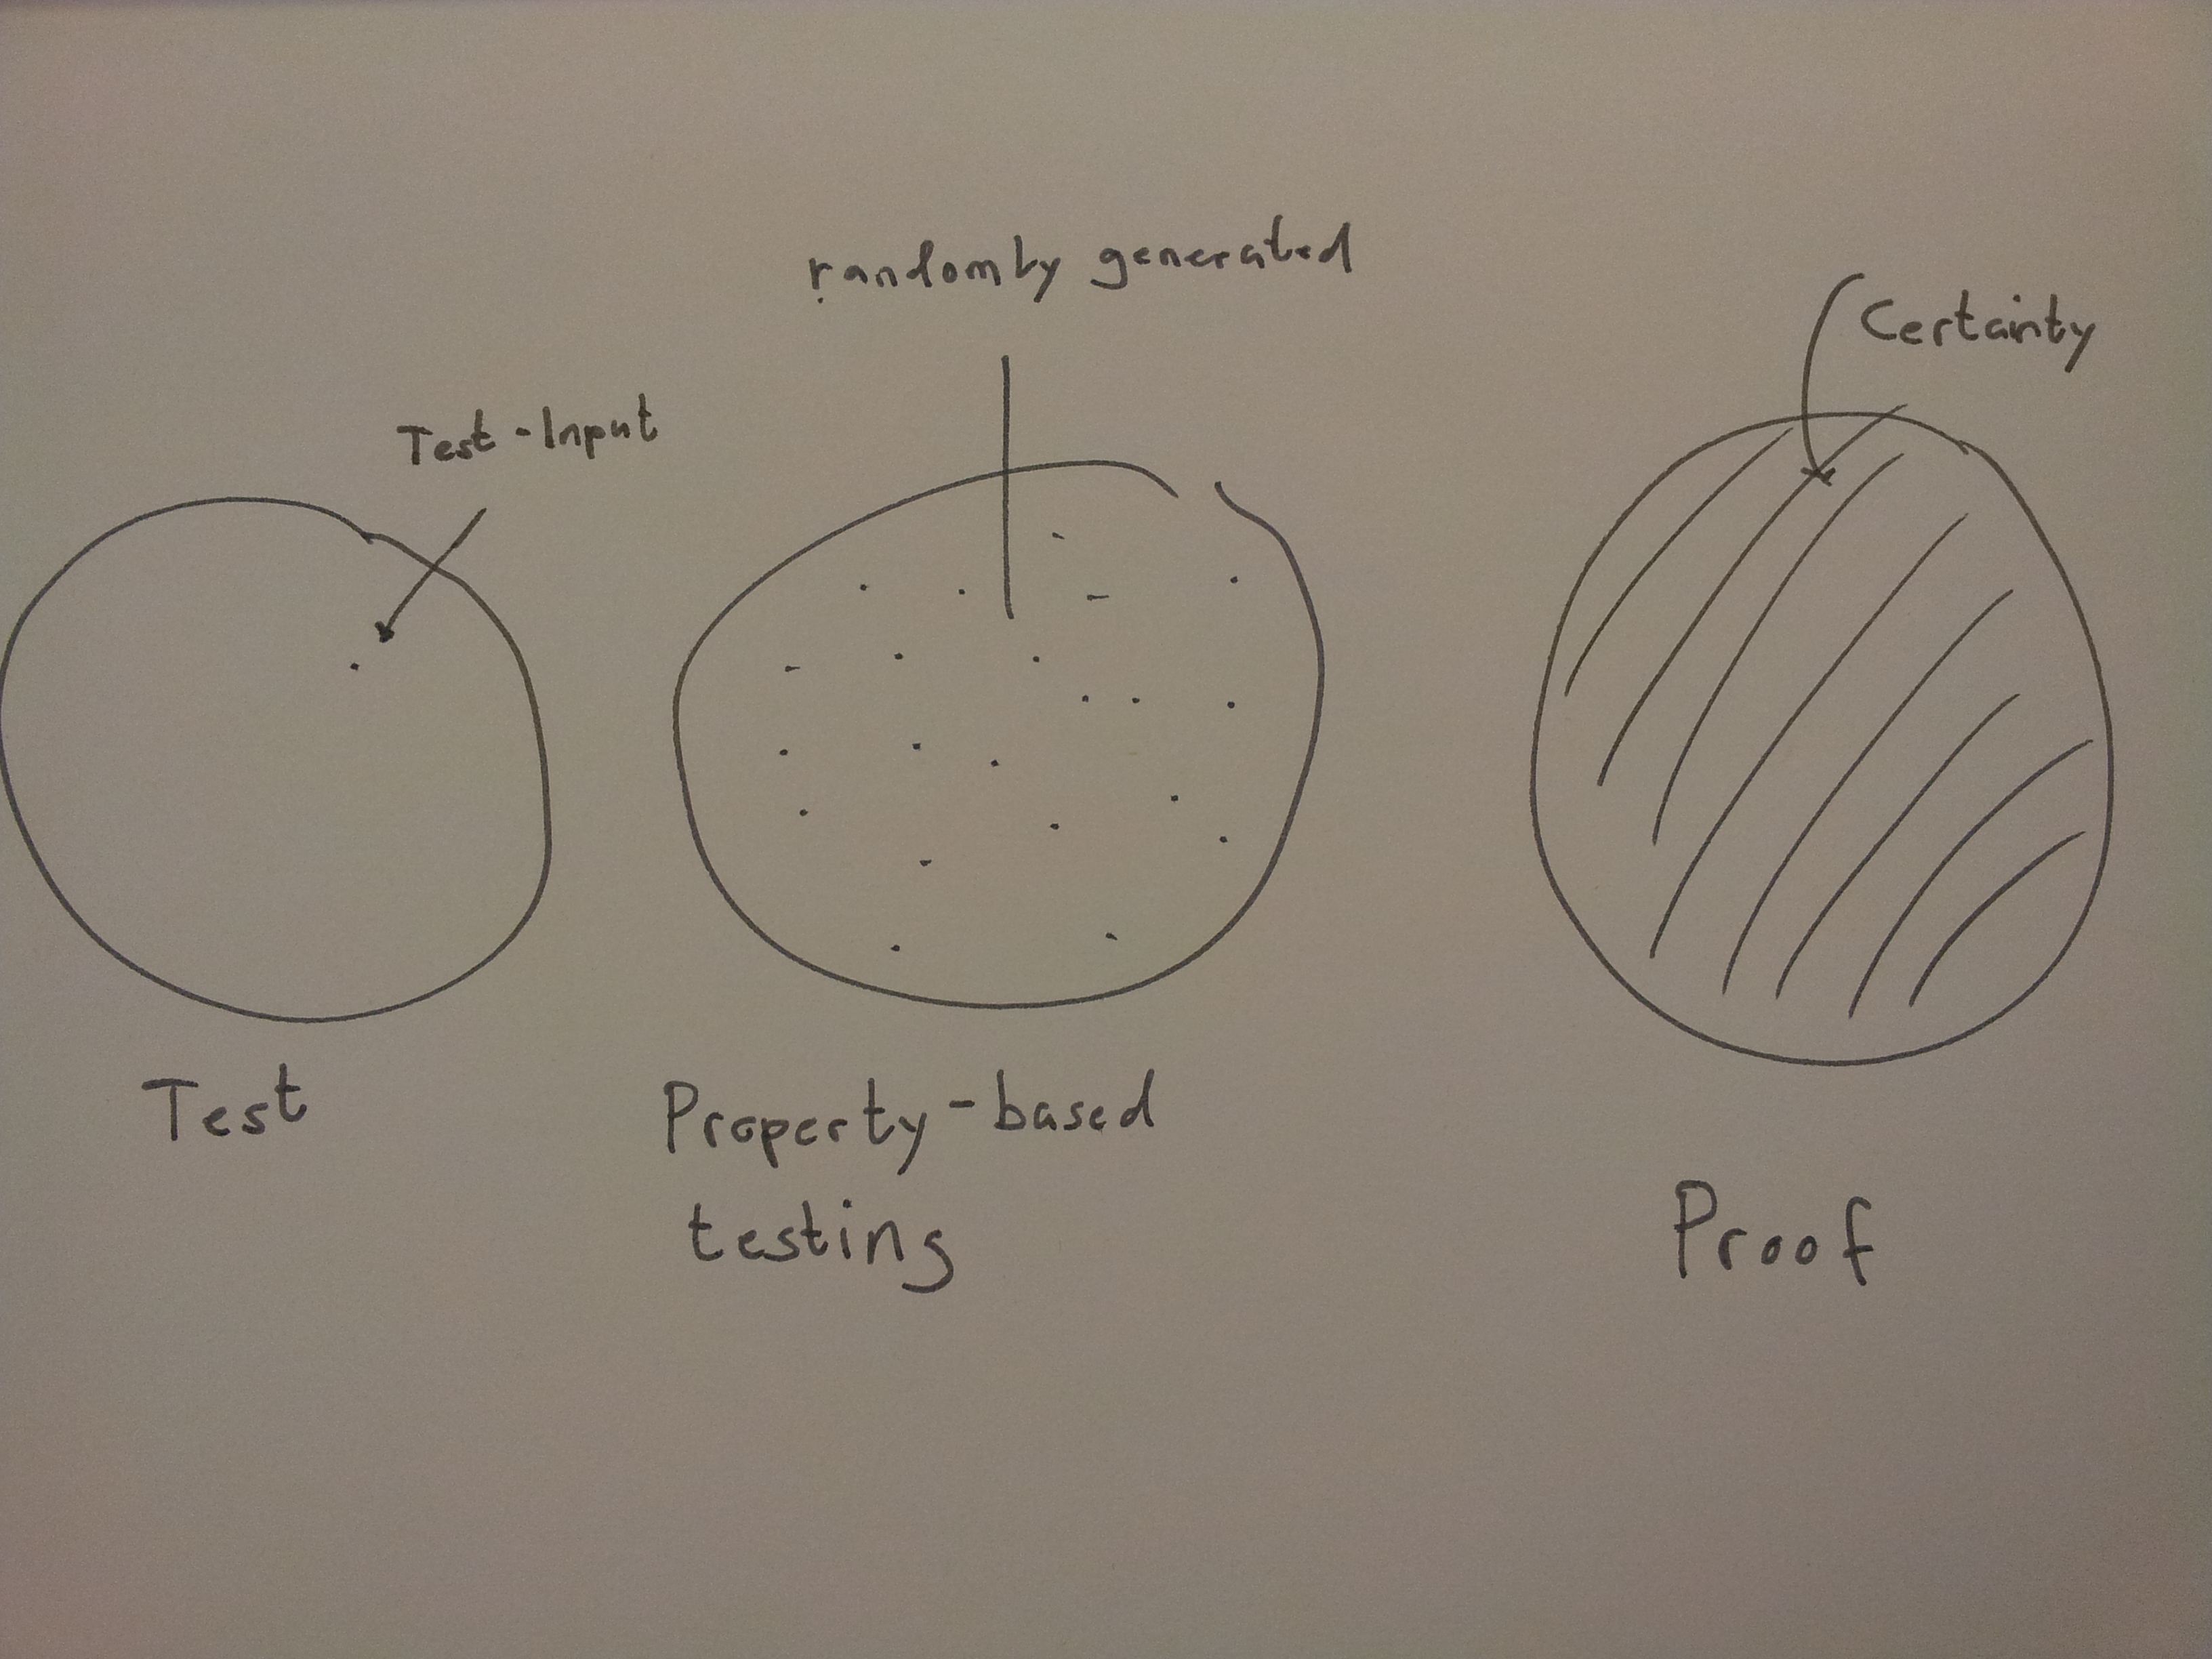
\includegraphics[width=0.9\textwidth]{comp}
  \caption{Comparison of test, property-based-testing and proof}
  \label{fig:property_validation}
\end{figure}

Equational reasoning isn't a method only used in programming. Equational reasoning is the process of substituting expressions. With equational reasoning we are able to show that certain properties hold.
For example, it's possible to show that
\begin{equation}
  \label{eq:sum}
  (x+a)(x+b) = x^2 + (a+b)x+ab
\end{equation}
is true. To show the equality we have to only have to substitute the expression on the left-hand side with the help of the basic algebraic properties of numbers (commutative, associative, distributive).

A function definition in Haskell means that we can substitute the lefthand side. Hence, we can use reasoning about a Haskell program in the same way, we reason about mathematical expressions. With equational reasoning it's possible to deduce properties from definitions.

For example, it's possible to show that 
\begin{program}
\end{program}

\section{Function composition}
\label{sec:functioncomposition}

Function composition in mathematics is defined as
\begin{equation}
  \label{eq:functioncomposition}
  (f \circ g)(x) = f(g(x))
\end{equation}

Haskell functions can be compose with the \verb|.| function.

\begin{figure}
  \centering
\begin{verbatim}
(.) :: (b -> c) -> (a -> b) -> a -> c
f . g = \x -> f (g x)
\end{verbatim}
  \caption{. function}
  \label{fig:compositionfunction}
\end{figure}

Function composition allows us to create a function by composing it with many small functions. 

Functions in Haskell form a category in category theory. They satisfy the category laws.
\begin{description}
\item[Associativity law] 
\item[Left/Right Identity law] 
\end{description}

\bibliographystyle{plain}
\bibliography{a}
\end{document}